\documentclass[a4paper,12pt]{report}

\usepackage[utf8]{inputenc}
\usepackage[T1]{fontenc}
\usepackage[italian]{babel}
\usepackage{geometry}
\usepackage{lmodern}
\usepackage{graphicx}
\usepackage{float}
\usepackage{tabularx}
\usepackage[table]{xcolor}
\usepackage{fancyvrb} 
\usepackage{alltt}
\usepackage{hyperref}

\geometry{margin=1in}

\hypersetup{
    colorlinks=false,
    pdfborder={1 1 1},
    linkbordercolor={1 0 0},
    urlbordercolor={1 0 0},
    citebordercolor={1 0 0},
    pdftitle={Elaborato Basi di Dati},
    pdfauthor={Maisam Noumi, Alessandro Rebosio, Filippo Ricciotti}
}

\usepackage[italian]{cleveref}

\title{
    \vspace*{2cm}
    \Huge\textbf{Agriturismo} \\[0.5cm]
    \LARGE Relazione per il corso di \\[0.2cm]
    \textit{Basi di Dati} \\[2cm]
}

\author{
    \Large
    Maisam Noumi \\
    Alessandro Rebosio \\
    Filippo Ricciotti
}

\date{
    \vspace{1cm}
    \today \\[0.5cm]
    Anno Accademico 2024-2025
}


\begin{document}


\maketitle

\tableofcontents

\chapter{Analisi dei requisiti}
Si ha come obiettivo la realizzazione di un database per la gestione di un agriturismo che offre un'ampia gamma di servizi: ristorazione,
ospitalità, piscina, attività con animali, sport e molto altro. A seguito dell'intervista è stata prodotta la seguente
descrizione delle specifiche del sistema in linguaggio naturale.

\section{Intervista}
\textit{L'agriturismo "Campo Verde" offre una vasta gamma di servizi, tra cui ospitalità, ristorazione, piscina, attività con animali
	e sport, e necessita di un sistema integrato per la gestione delle prenotazioni, dei clienti e delle attività.}

\textit{Il sistema dovrà gestire diverse tipologie di servizi, tra cui camere, tavoli al ristorante, lettini in piscina, attività
	con animali e campo da calcio. Ogni servizio avrà regole specifiche: ad esempio, i lettini in piscina sono prenotabili per fasce orarie
	di 2 ore, mentre il campo da calcio può essere prenotato per un'ora o più.}

\textit{Per ogni cliente verranno memorizzati nome, cognome, codice fiscale, indirizzo email e numero di telefono. Al momento della
	registrazione, verrà creato un account personale con credenziali di accesso alla piattaforma. Ogni cliente potrà effettuare prenotazioni
	solo se autenticato, e ogni prenotazione verrà registrata con i relativi dettagli (servizio richiesto, data, orario e numero di partecipanti).}

\textit{I clienti potranno acquistare sia servizi singoli che pacchetti combinati, creati dallo staff o personalizzati in base alle
	loro esigenze. Ogni pacchetto potrà includere più servizi (es. pernottamento + cena + attività con animali) e avrà un prezzo
	specifico, con eventuali sconti applicabili in base alla stagione o a promozioni speciali.}

\textit{Ogni prenotazione verrà confermata via email, con la possibilità di modificarla o cancellarla entro un certo termine. In
	caso di mancata presentazione senza preavviso, potrà essere applicata una penale. Le prenotazioni per eventi speciali (come tornei o cene a tema)
	richiederanno spesso un acconto non rimborsabile.}

\textit{L'agriturismo terrà traccia di tutte le prenotazioni effettuate dai clienti, mantenendo uno storico che permetterà
	di analizzare le preferenze e di proporre offerte personalizzate. I clienti potranno lasciare recensioni per ogni servizio utilizzato, valutandolo
	con un voto da 1 a 5 stelle e aggiungendo un commento. Le recensioni verranno moderate dallo staff e potranno essere utilizzate per
	migliorare i servizi offerti.}

\textit{Il sistema permetterà anche la gestione degli eventi organizzati dall'agriturismo, come tornei di calcio o laboratori con animali. Per ogni
	evento sarà possibile definire il numero massimo di partecipanti, il prezzo e le date disponibili. I clienti potranno iscriversi agli eventi direttamente
	dalla piattaforma, ricevendo una conferma e i dettagli organizzativi.}

\textit{Lo staff dell'agriturismo avrà accesso a una dashboard che mostrerà in tempo reale lo stato delle prenotazioni, l'occupazione delle
	camere e dei servizi, e le recensioni ricevute. Potranno generare report periodici per analizzare l'andamento delle prenotazioni, le preferenze dei clienti e
	l'efficacia delle promozioni. Inoltre, il sistema supporterà la gestione di account multipli per lo staff, con diversi livelli di accesso in base al
	ruolo (es. receptionist, responsabile del ristorante, gestore della piscina).}

\section{Prima fase di analisi}
A seguito di un'analisi preliminare dei requisiti, sono emerse alcune aree critiche che necessitano di specifiche tecniche
aggiuntive. Per colmare queste lacune informative, è stato condotto un ciclo di interviste mirate con i gestori dell'agriturismo, i
cui esiti sono sintetizzati nella tabella seguente:

\paragraph{D:}
“Come devono essere gestite le prenotazioni, dalla loro creazione alla cancellazione?”
\\ {\bf R:} “Le prenotazioni possono essere effettuate tramite il sito web, telefonicamente o direttamente in reception. Ogni servizio avrà un termine
entro il quale è possibile modificare o cancellare la prenotazione senza penali. Per le camere, ad esempio, la cancellazione è gratuita fino a 48 ore prima
dell'arrivo. Per i servizi a tempo, come il campo da calcio, la cancellazione è possibile fino a 24 ore prima.”

\paragraph{D:}
“Come devono essere gestiti i pacchetti combinati?”
\\ {\bf R:} “I pacchetti possono essere creati dallo staff con servizi predefiniti. Ogni pacchetto avrà un prezzo complessivo calcolato in base ai
servizi inclusi, con eventuali sconti applicati.

\newpage
\section{Estrazione dei concetti principali}
Dall'analisi svolta emergono le principali entità che il sistema dovrà gestire: \textbf{Cliente}, \textbf{Servizio}, \textbf{Prenotazione},
\textbf{Pacchetto}, \textbf{Evento}, \textbf{Recensione} e \textbf{Staff}.

Ogni \textbf{Cliente} potrà registrarsi fornendo i seguenti attributi: \newline \underline{nome}, \underline{cognome}, \underline{codice fiscale},
\underline{email} e \underline{numero di telefono}. All'atto della registrazione, verrà creato un account contenente \underline{username} e \underline{password}. Solo i clienti
autenticati potranno effettuare prenotazioni. Ogni cliente avrà accesso al proprio \underline{storico prenotazioni} e potrà lasciare recensioni.

I \textbf{Servizi} gestiti comprendono: \underline{camere}, \underline{tavoli ristorante}, \newline \underline{lettini piscina}, \underline{attività con
	animali} e \underline{campo da calcio}. Ogni servizio presenta regole specifiche: ad esempio, i lettini in piscina sono prenotabili a fasce orarie di
due ore, mentre il campo da calcio è prenotabile per una o più ore. Per ciascun servizio devono essere definiti \underline{orari}, \underline{capacità massima},
\underline{durata prenotabile} e \underline{penali in caso di cancellazione}.

La \textbf{Prenotazione} sarà associata a un cliente e a uno o più servizi, e includerà \underline{data}, \underline{orario}, \underline{numero di
	partecipanti} e \underline{stato}. La cancellazione sarà possibile secondo i termini previsti (es. 48 ore per le camere, 24 per servizi a tempo). In caso di
mancata presentazione, potrà essere applicata una \underline{penale}, mentre per eventi speciali sarà richiesto un \underline{acconto non rimborsabile}.

Il sistema gestirà anche \textbf{Pacchetti}, ovvero combinazioni \newline di più servizi, con un \underline{prezzo complessivo},
eventuali \underline{sconti promozionali} e possibilità \newline di \underline{personalizzazione}. I pacchetti potranno essere creati dallo staff o richiesti dai clienti.

Per quanto riguarda gli \textbf{Eventi}, come tornei o laboratori, saranno definiti con \underline{nome}, \newline \underline{descrizione}, \underline{data},
\underline{prezzo}, \underline{numero massimo di partecipanti} e, se necessario, \underline{acconto}. I clienti potranno iscriversi online e riceveranno conferma via email.

Le \textbf{Recensioni} potranno essere lasciate dai clienti solo dopo aver usufruito di un servizio. Ogni recensione includerà
una \underline{valutazione da 1 a 5 stelle} e un \underline{commento testuale}. Le recensioni verranno \underline{moderate} dallo staff prima della pubblicazione.

Lo \textbf{Staff} accederà al sistema tramite un \underline{account personale} con \underline{ruolo} definito (es. receptionist, gestore piscina). Tramite
una \underline{dashboard}, lo staff potrà monitorare in tempo reale le \underline{prenotazioni}, lo \underline{stato di occupazione dei servizi} e le
\underline{recensioni}. Il sistema permetterà inoltre la \underline{generazione di report} statistici sull'attività dell'agriturismo.


\chapter{Preogettazione concettuale}
In questo capitolo presenteremo lo schema ER, partendo da una versione iniziale e migliorandola passo dopo passo final ad arrivare a quella
definitiva, attraverso dei raffinamenti

\section{Schema scheletro}
Dopo aver eseguito l'analisi del dominio iniziale, abbiamo creato uno schema di base con le entità e le relazioni principali,
che sarà poi perfezionato nei passaggi successivi.
\begin{figure}[H]
	\centering
	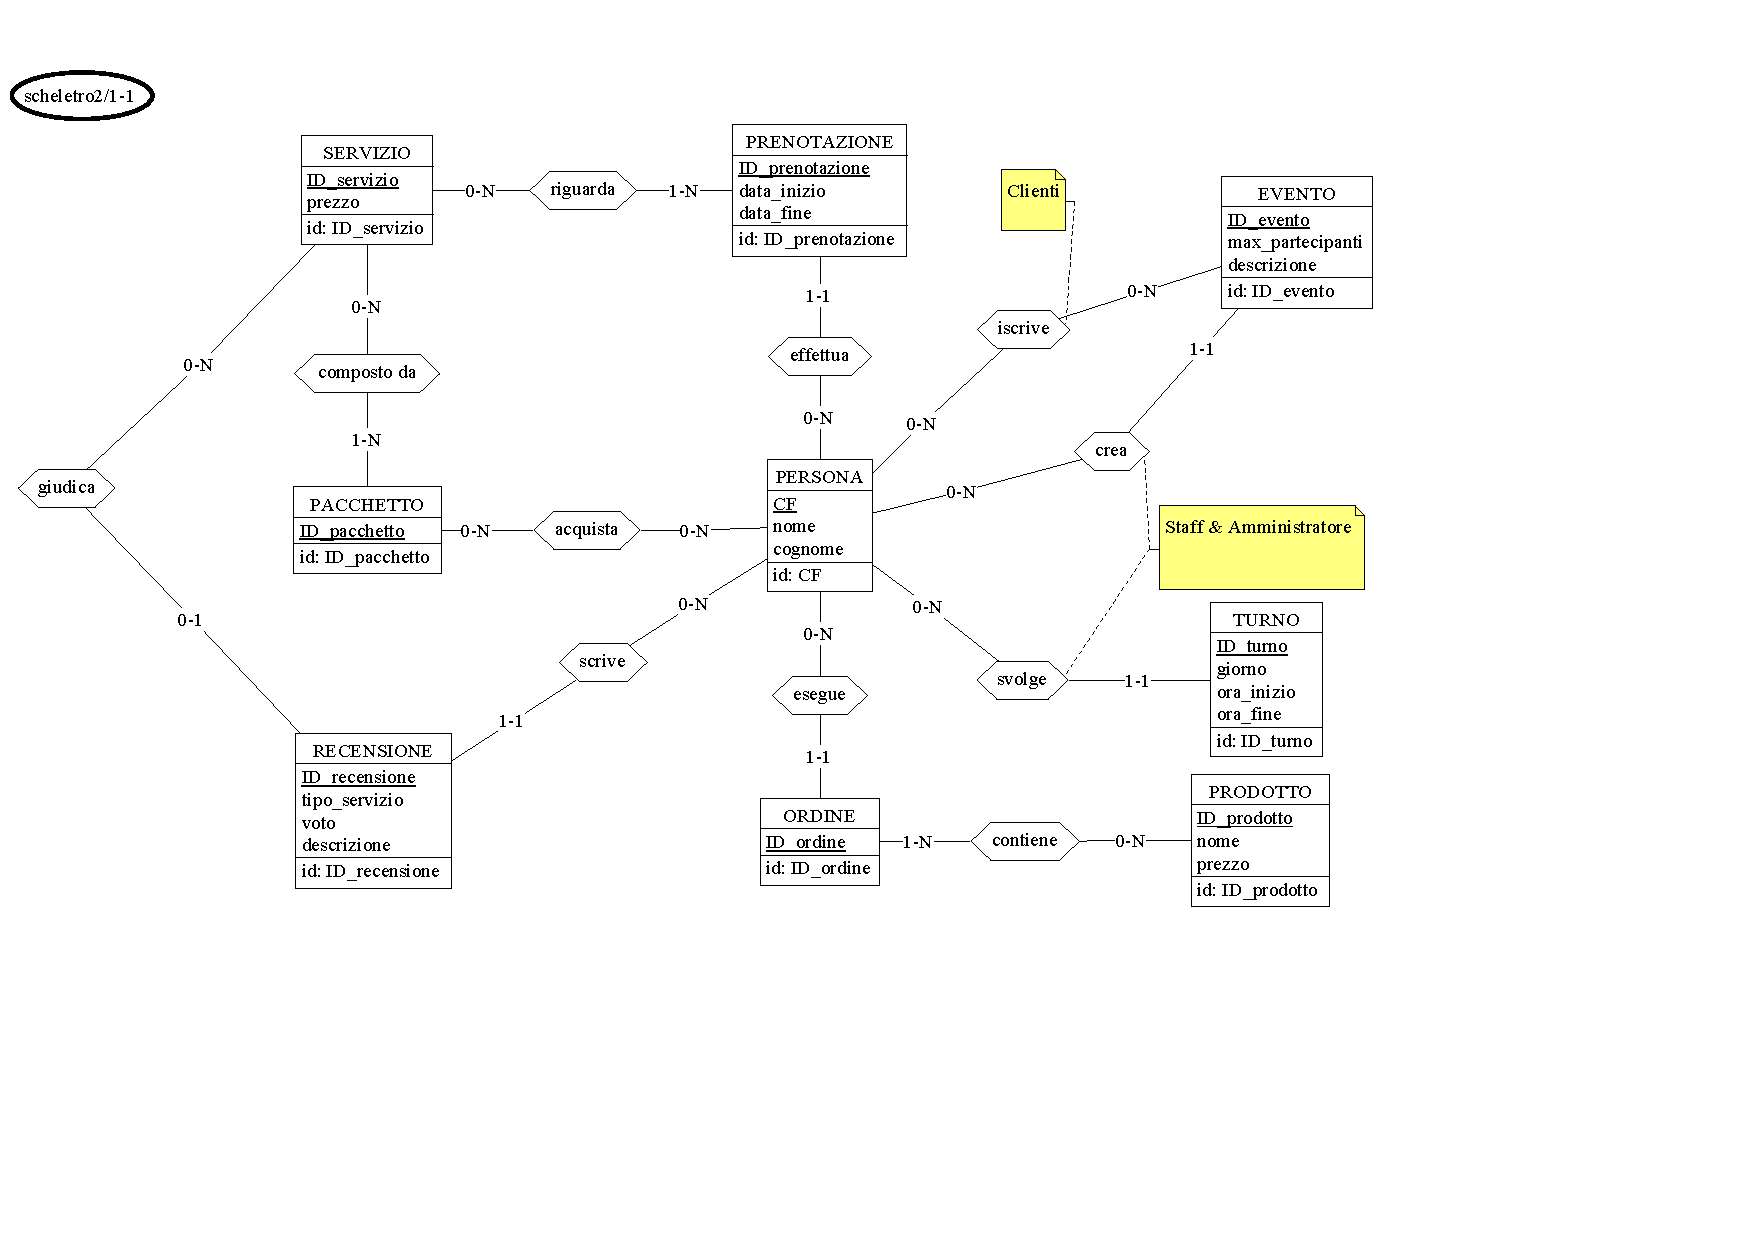
\includegraphics[width=\textwidth, trim=0 100pt 150pt 0 , clip]{./pdf/scheletro.pdf}
	\caption{Schema ER scheletro (versione iniziale)}
	\label{fig:schema-scheletro}
\end{figure}

\section{Raffinamenti proposti}
\subsection{Utente e Dipendente}
Nel modello concettuale iniziale \textbf{Persona} accorpava in sé tutte le possibili iterazioni con il sistema: iscrizione e creazione
di eventi, acquisto di pacchetti, prenotazioni, ordini e recensioni. Questo apporccio, sebbene corretto sul piano logico, risultava poso chiaro
perché attribuiva a un'unica entità responsabilità moltoterogenee.

\vspace{\baselineskip}
Per migliorare la rappresentazione è stato introdotto un rafinameto
attraverso un'operazione di \textbf{generalizzazione/specializzazione}: la superclasse \textbf{Persona} è stata mantenuta
per raccogliere gli attributi comuni (CF, nome, cognome), mentre le funzionalità specifiche sono state distribuite nei sottotipi
\textbf{Cliente} e \textbf{Dipendente}.

\vspace{\baselineskip}
In questo modo i clienti gestiscono attività come acquisti, recensioni, ordini e iscrizioni agli eventi, mentre
i dipendenti si occupano dellac creazione degli eventi e della gestione dei servizi. Tale raffinamento migliora
la chiarezza semantica del modello, evita ambiguità e riflette meglio la separazione dei ruoli reali all'interno
del dominio applicativo.

\begin{figure}[H]
	\centering
	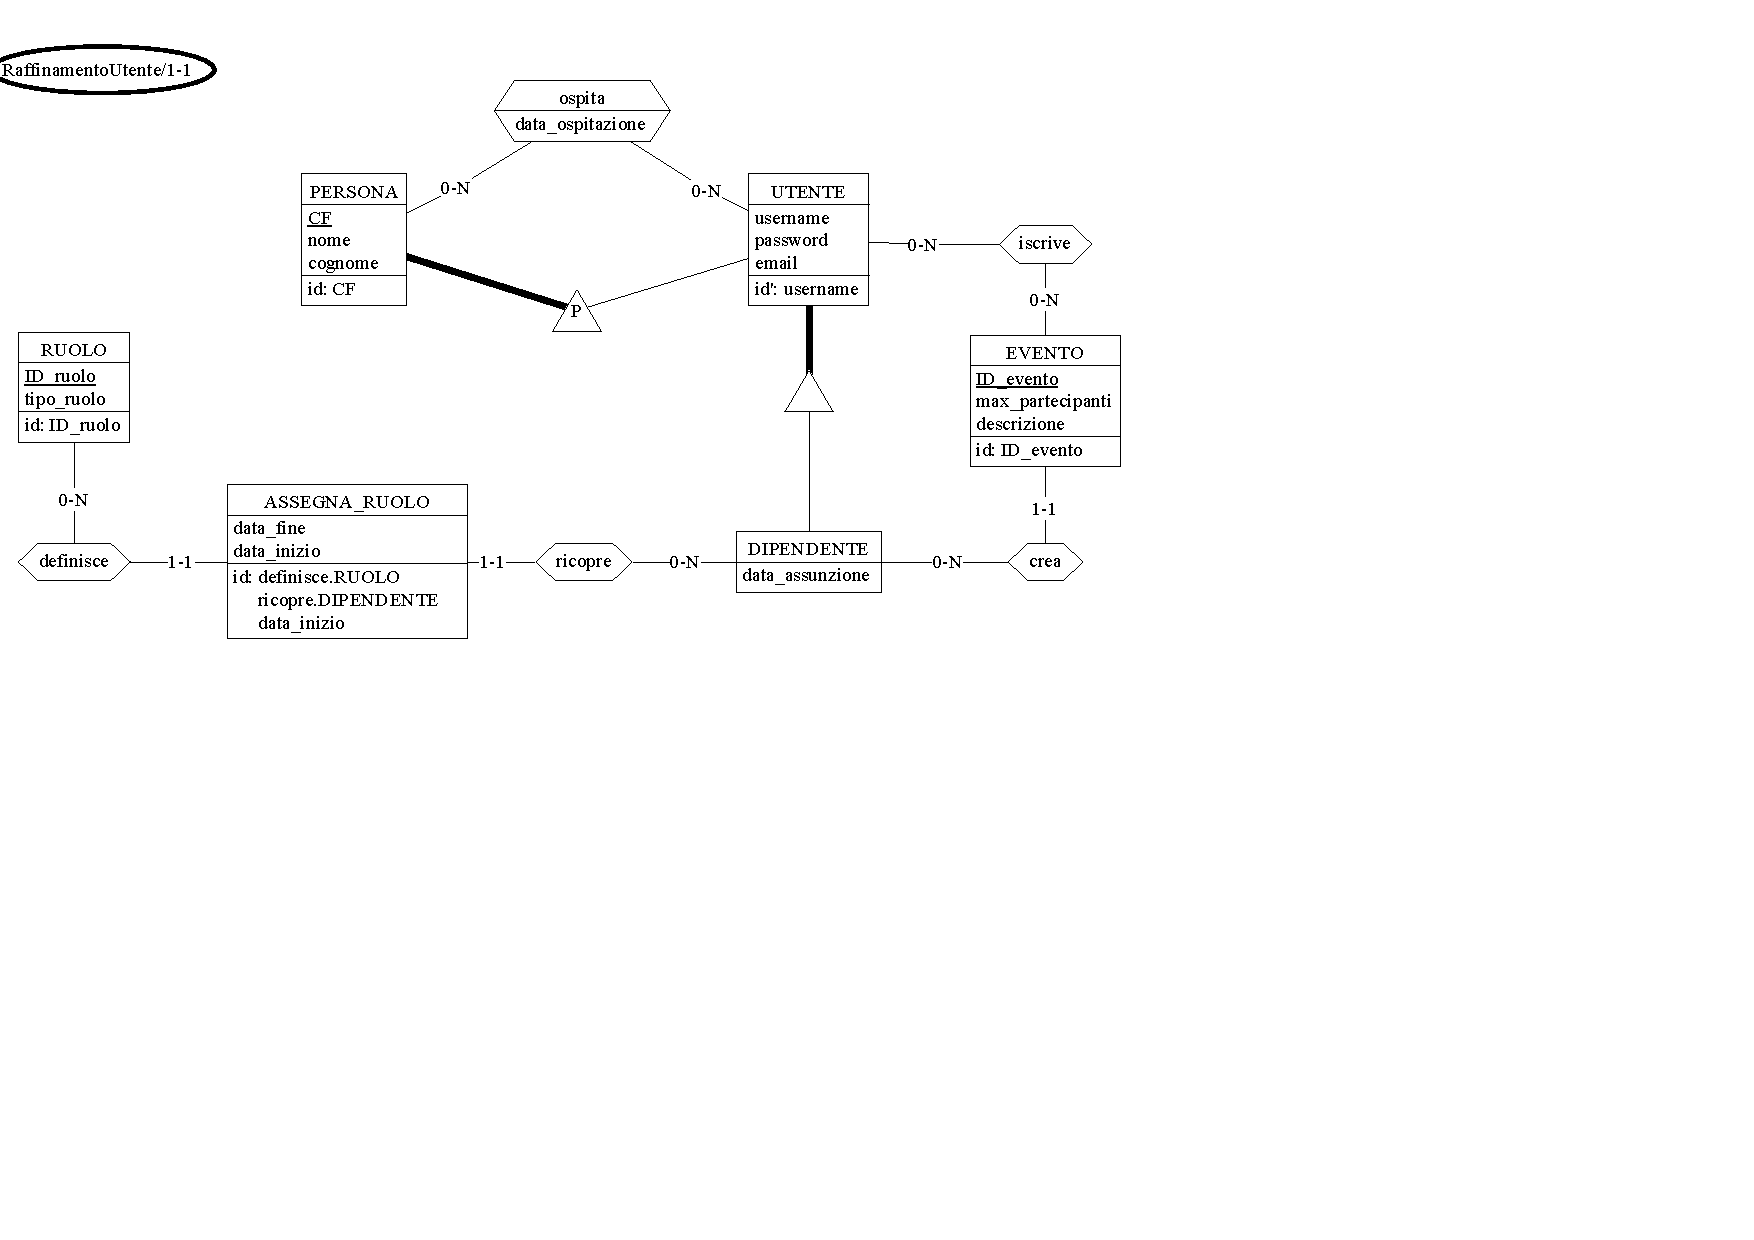
\includegraphics[width=\textwidth, trim=0 250pt 300pt 0, clip]{./pdf/raffinamento utente.pdf}
	\caption{Schema ER, raffinamento utente}
	\label{fig:raffinamento-utente}
\end{figure}

\newpage
\subsection{Servizi/Prenotazioni e Pacchetti}
Nel modello iniziale i diversi tipi di servizi (camere, tavoli, lettini, campi da gioco, attività con animali) potevano essere
rappresentati come entità distinte, con il rischio però di ridondanza e frammentazione dei dati.

\vspace{\baselineskip}
Con il raffinamento si è introdotta una \textbf{generalizzazione}: è stata creata la superclasse \textbf{Servizio}, che raccoglie gli attributi comuni (ID\_servizio,
prezzo, tipo\_servizio, status), mentre ciascuna tipologia specifica di servizio (Camera, Tavolo, Lettino, Campo da gioco,
Attività con animali) è modellata come sottoclasse.

\vspace{\baselineskip}
Inoltre, è stato introdotto il legame con l'entità \textbf{Prenotazione}, che consente di registrare le informazioni su data di inizio
e fine e di associare ogni prenotazione a uno o più servizi specifici tramite la relazione con \textbf{Dettagli Prenotazione}. Questo
raffinamento permette di gestire correttamente scenari in cui un utente prenota più servizi differenti nello stesso arco
temporale.

\vspace{\baselineskip}
Infine, i \textbf{Pacchetti} offrono un ulteriore livello di astrazione: ciascun pacchetto è composto da uno o più servizi e può essere
acquistato dall'utente come un'unica offerta integrata. L'introduzione dei pacchetti, combinata con le prenotazioni, permette
di modellare sia l'acquisto di singoli servizi che la sottoscrizione di offerte composte, rendendo il sistema più flessibile e
vicino a un contesto reale.

\begin{figure}[H]
	\centering
	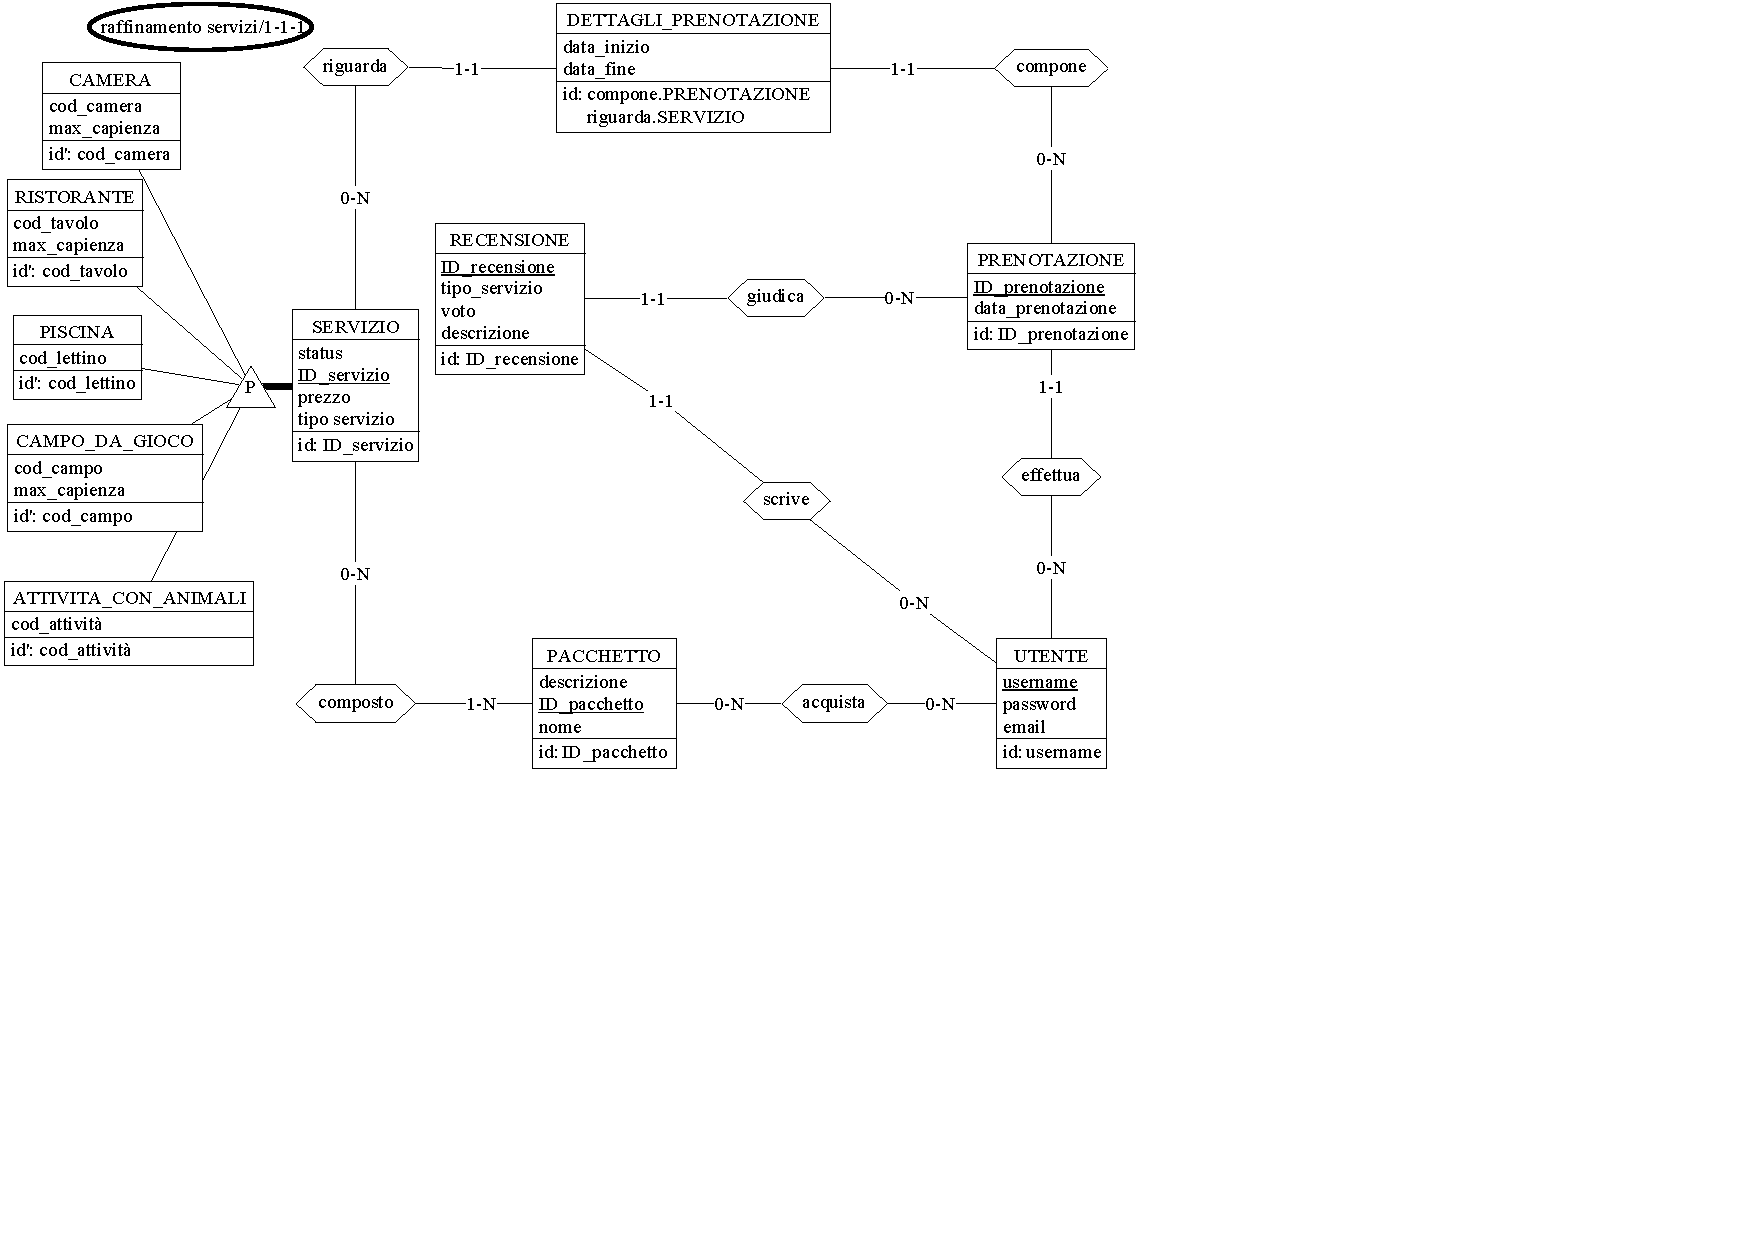
\includegraphics[width=\textwidth, trim=0 200pt 175pt 0, clip]{./pdf/raffinamento servizi.pdf}
	\caption{Schema ER, raffinamento servizi}
	\label{fig:raffinamento-servizi}
\end{figure}

\newpage
\subsection{Prodotti e ordini}
Nel modello concettuale iniziale, la gestione degli ordini e dei prodotti risultava poco dettagliata: un ordine era
semplicemente collegato a uno o più prodotti, senza possibilità di specificare informazioni aggiuntive come quantità o
prezzo unitario.

\vspace{\baselineskip}
Con il raffinamento, è stata introdotta l'entità \textbf{Dettaglio Ordine}, che funge da associazione tra \textbf{Ordine}
e \textbf{Prodotto}. Ogni dettaglio ordine consente di memorizzare, per ciascun prodotto incluso in un ordine, la quantità
acquistata e il prezzo applicato. Questo permette di rappresentare in modo accurato scenari reali come ordini
multiprodotto, applicazione di sconti o variazioni di prezzo nel tempo.

\vspace{\baselineskip}
Inoltre, viene mantenuta la generalizzazione tra \textbf{Persona} e \textbf{Utente}, già introdotta nei raffinamenti
precedenti, per distinguere i dati anagrafici comuni da quelli specifici per l'accesso al sistema e la gestione degli
ordini. Questo approccio migliora la flessibilità e la chiarezza del modello, consentendo una gestione più efficace
delle informazioni relative agli acquisti.

\begin{figure}[H]
	\centering
	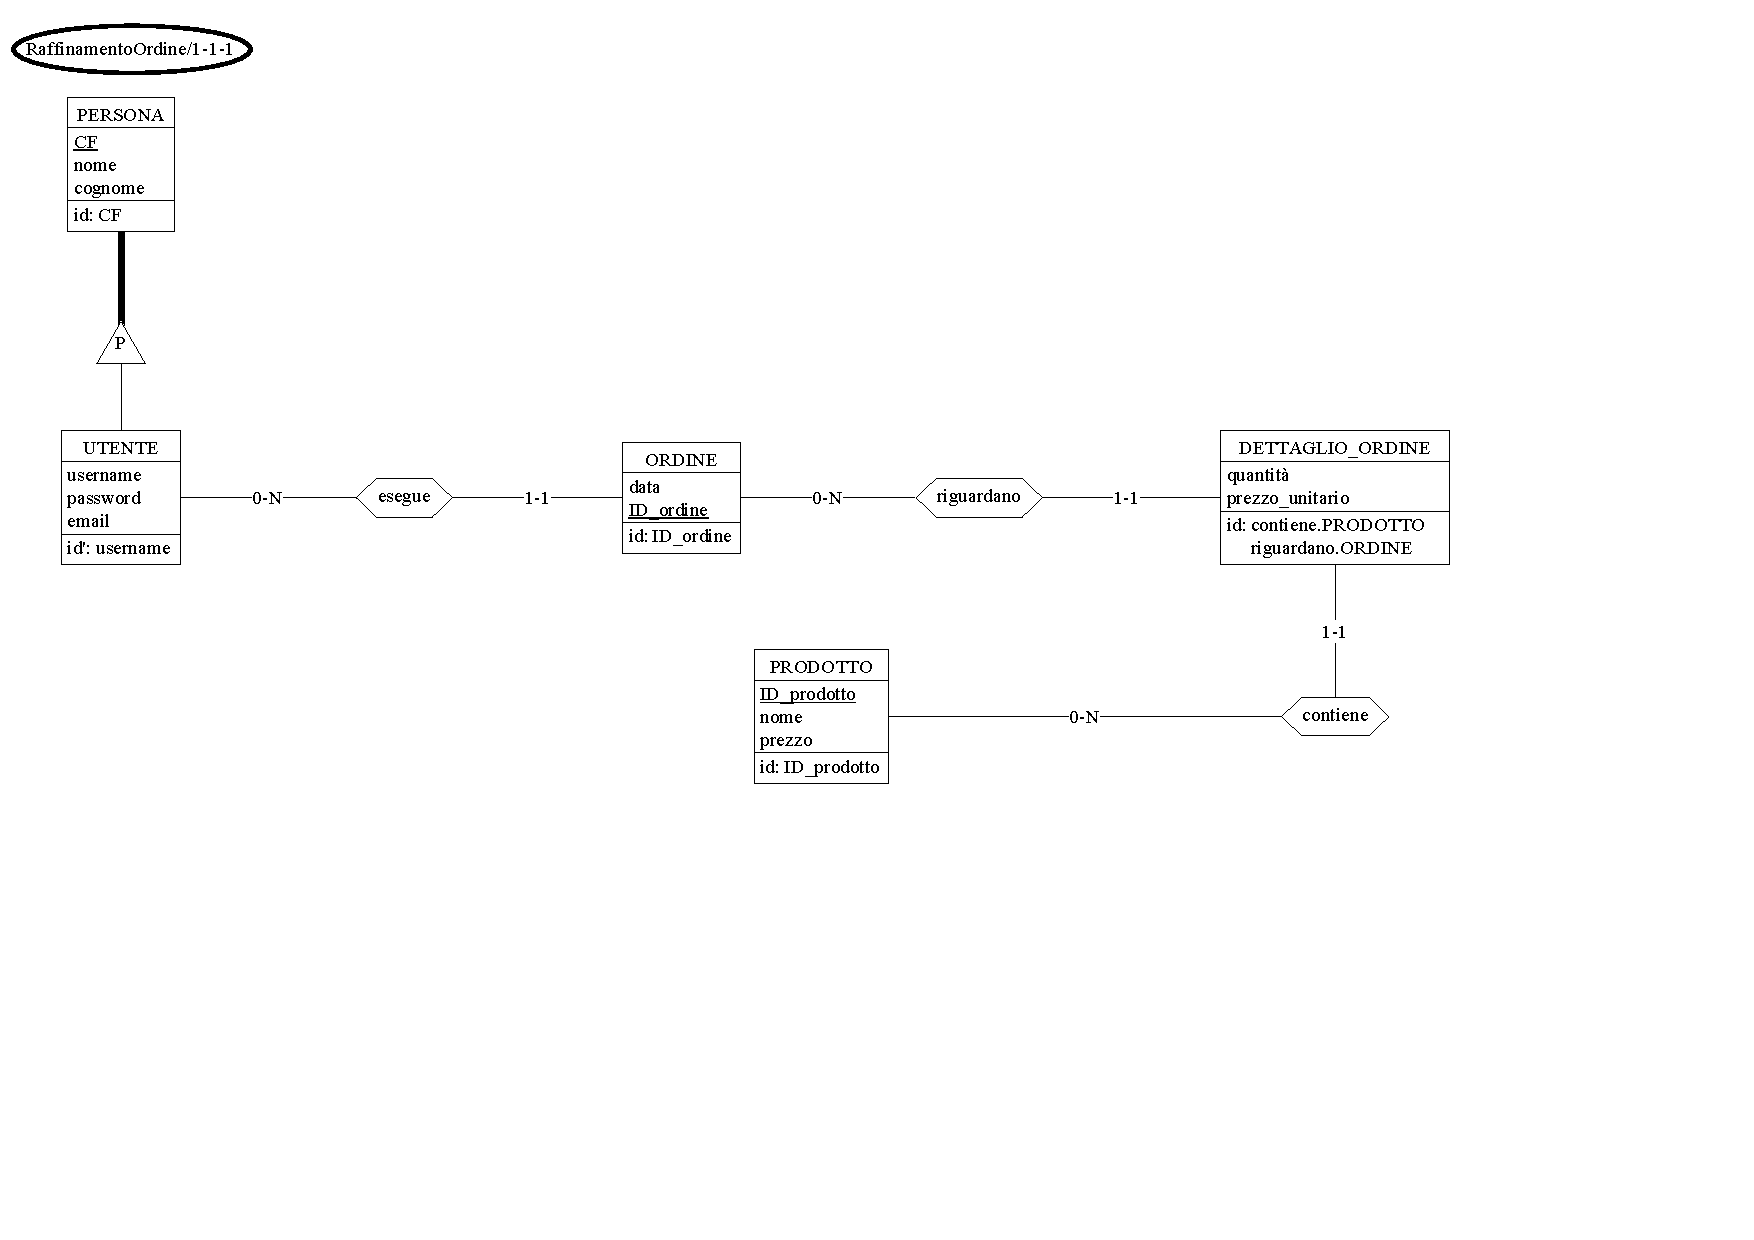
\includegraphics[width=\textwidth, trim=0 200pt 125pt 0, clip]{./pdf/raffinamento prodotto.pdf}
	\caption{Schema ER, raffinamento prodotto}
	\label{fig:raffinamento-prodotto}
\end{figure}

\newpage
\section{Schema concettuale finale}
Qui di seguito, è presente lo schema concettuale finale con tutti i raffinamenti.

\begin{figure}[H]
	\centering
	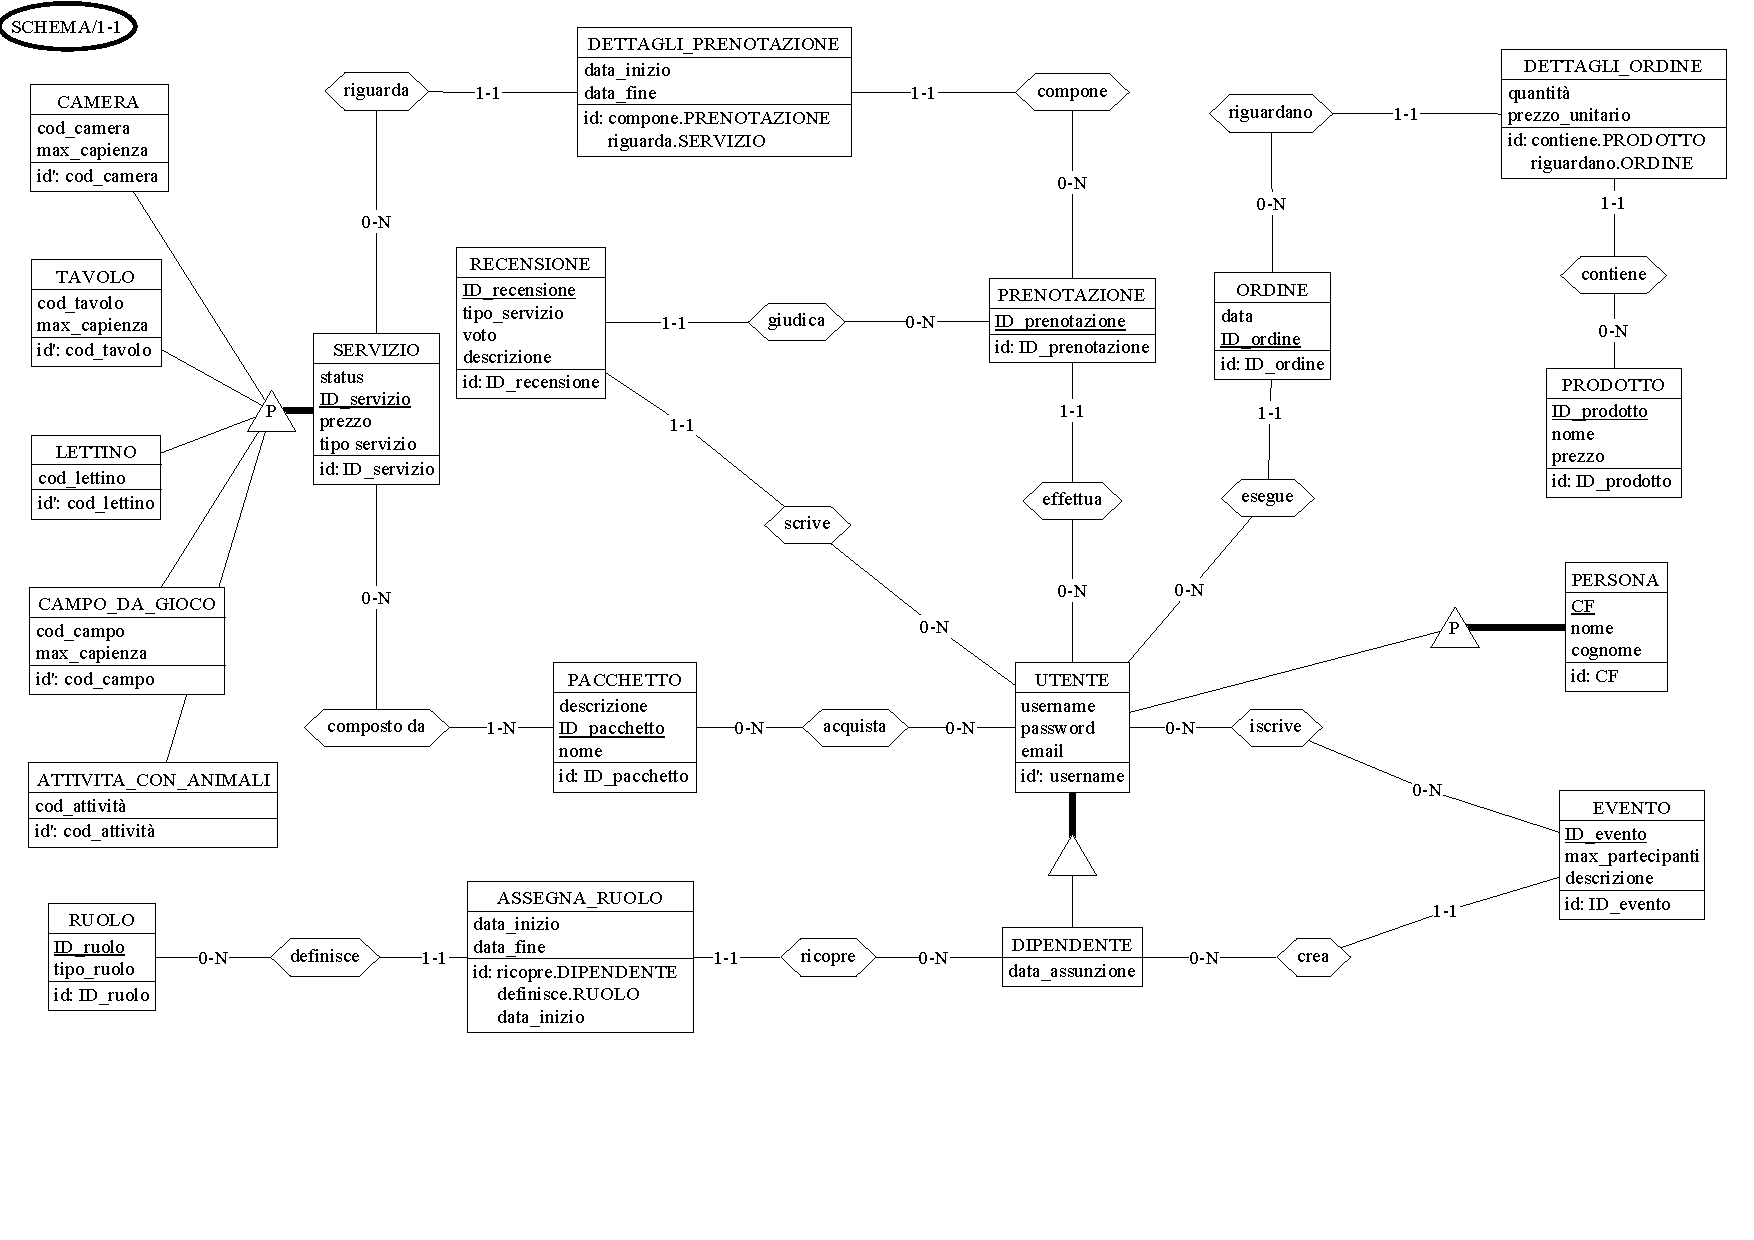
\includegraphics[width=\textwidth, trim=0 100pt 0 0, clip, angle=0]{./pdf/finale.pdf}
	\caption{Schema ER, schema concettuale finale}
	\label{fig:schema-finale}
\end{figure}
\newpage

\chapter{Progettazione logica}
\section{Stima del volume dei dati}
Per poter far un'ottima progettazione, è stata creata una stima della qunatità dei dati, che il database dovrà gestire. La stima
è stata calcolata considerando un agriturismo di medie dimensioni, con circa 20 camere, un ristorante e attività all'aperto.

\begin{table}[H]
	\centering
	\small
	\renewcommand{\arraystretch}{1.15}
	\begin{tabularx}{\textwidth}{|l|c|c|X|}
		\hline
		\rowcolor{gray!20}
		\textbf{Tabella}     & \textbf{E/A} & \textbf{Stima record} & \textbf{Note}                                          \\
		\hline
		persona              & E            & 1000                  & Clienti e dipendenti storicizzati                      \\
		utente               & E            & 500                   & Account di accesso (clienti e staff)                   \\
		dipendente           & E            & 20                    & Dipendenti attivi e storici (subset di utente)         \\
		ruolo                & E            & 5                     & Tipologie di ruolo (receptionist, amministratore, ...) \\
		assegna ruolo        & A            & 30                    & Storico assegnazioni ruolo (associazione)              \\
		pacchetto            & E            & 30                    & Pacchetti promozionali / stagionali                    \\
		servizio             & E            & 50                    & Camere, tavoli, lettini, campi, attività               \\
		camera               & E            & 20                    & Specializzazione di servizio: camere                   \\
		tavolo               & E            & 10                    & Specializzazione di servizio: tavoli ristorante        \\
		campo da gioco       & E            & 2                     & Specializzazione di servizio: campi sportivi           \\
		lettino              & E            & 15                    & Specializzazione di servizio: lettini piscina          \\
		attivita con animali & E            & 3                     & Attività guidate con animali                           \\
		composto da          & A            & 100                   & Associazione pacchetto-servizio                        \\
		\hline
	\end{tabularx}
	\caption{Stima del volume dei dati per le tabelle definite in farmhouse.sql}
\end{table}

\section{Descrizione operazioni}
In questa sezione vengono riportate le principali operazioni che saranno svolte sulla base di dati.
Si è stimata la frequenza con cui ogni operazione viene eseguita in media, nell'arco di una settimana,
specificando anche il tipo di utente che la effettua e il tipo di accesso al DB (letture/scritture).

\section{Analisi delle operazioni}
Di seguito viene riportata un'analisi per alcune delle operazioni principali sul database dell'agriturismo.

\begin{enumerate}
	\item Registrazione nuovo utente
	\item Prenotazione servizi
	\item Creazione pacchetto
	\item Modifica/cancellazione prenotazione
	\item Acquisto pacchetto
	\item Inserimento recensione
	\item Inserimento oridne prodotti
	\item Iscrizione evento
	\item Inserimento ordine prodotti
\end{enumerate}

\section{Analisi delle ridondanze}

\section{Riepilogo operazioni}

\section{Raffinamento dello schema}

\section{Schema relazionale finale}

\chapter{Progettazione della Base di Dati}
\section{Traduzione delle operazioni}

\chapter{Progettazione dell'applicazione}


\end{document}
